\documentclass[a4paper,11pt]{article}

\usepackage[utf8]{inputenc}
\usepackage{booktabs}
\usepackage{hyperref}
\usepackage{listings}  
\usepackage{tikz}
\usepackage{float}
\usepackage{color}
\usepackage{hhline}
\usepackage{amsmath}
\usepackage{natbib}
\usepackage{epstopdf}
\usepackage{manual}
\usepackage[nottoc,numbib]{tocbibind}
\renewcommand\bibname{References}

\setcounter{tocdepth}{4}

\lstset{ 
  breaklines=true,          
}
\textwidth=450 pt
\hoffset = 0 pt
\marginparwidth = 0pt
\oddsidemargin = 0 pt

\newcommand{\HRule}{\rule{\linewidth}{0.5mm}}

\begin{document}
\begin{titlepage}
\begin{center}

% Title
\HRule \\[0.4cm]
{ \huge \bfseries PyFDAP: automated analysis of Fluorescence Decay After Photoconversion (FDAP) experiments\\[0.4cm] 
User Guide \\[0.4cm] }

\HRule \\[1.5cm]

\large
Alexander Bl\"a\ss le and Patrick M\"uller\\[0.5cm]

Friedrich Miescher Laboratory of the Max Planck Society\\
Spemannstra\ss e 39\\
72076 T\"ubingen\\
Germany\\[0.5cm]

E-Mail: \href{mailto:alexander.blaessle@tuebingen.mpg.de}{alexander.blaessle@tuebingen.mpg.de}, \href{mailto:patrick.mueller@tuebingen.mpg.de}{patrick.mueller@tuebingen.mpg.de}\\
Website: \href{http://people.tuebingen.mpg.de/mueller-lab/}{http://people.tuebingen.mpg.de/mueller-lab/}

\vfill

\end{center}
\end{titlepage}

\tableofcontents
\newpage
\section{Introduction}
Fluorescence Decay After Photoconversion (FDAP) is a microscopy-based technique for measuring protein half-lives \citep{Rogers2014}. In FDAP experiments, a protein of interest is tagged with a photoconvertible fluorescent protein and expressed \textit{in vivo}. The fluorescent fusion protein is then photoconverted, and the decrease in fluorescence intensity over time is monitored. The resulting intensity data is fitted with a decay function, and half-lives can be calculated from the fits.

Both intracellular and extracellular protein half-lives can be determined using FDAP. A static intracellular signal (e.g. Alexa488-dextran) can be used to create an intracellular mask, such that only intracellular pixels are considered when calculating intracellular intensity. The mask can be inverted to calculate extracellular intensities. 

Here, we provide a standardized computational framework to analyze FDAP datasets. Our software PyFDAP features (i) a comprehensive data format for handling, sorting, and annotating large FDAP datasets, (ii) the capability to separate fluorescence intensities in FDAP datasets into intra- and extracellular compartments based on counter-labeling, (iii) established fitting algorithms, and (iv) a user-friendly environment that allows researchers from a non-computational background to easily evaluate FDAP datasets.

\section{Installation}

PyFDAP was developed as an open source graphical user interface (GUI) in Python with PyQT and SciPy in order to make it accessible and extendable across the most frequently used operating systems Ubuntu Linux, Mac OS X, and Microsoft Windows. Over the past two decades, Python has become a widely used scientific programming language and provides PyFDAP users with enormous resources and easily addable software packages \citep{Millman2011}. 

All software packages needed to run PyFDAP are freely available. PyFDAP can be installed using stand-alone executables (see Section~\ref{sec:executable}). Alternatively, users can run the PyFDAP packages from source (see Section~\ref{sec:source}), which offers the possibility to edit the PyFDAP code and to import new modules.

\subsection{Running PyFDAP using stand-alone executables}
\label{sec:executable}
Download the executable that fits your system from \href{http://people.tuebingen.mpg.de/mueller-lab/}{http://people.tuebingen.mpg.de/mueller-lab/}. This is suitable for users who want to analyze FDAP experiments and do not need to customize the PyFDAP code. A list of currently available binary files and systems on which the binaries have been tested can be found in Table \ref{tab:executables}. If there is no executable available for your system, we recommend using the Anaconda installation approach explained in Section~\ref{sec:anaconda}.
 
 \begin{table}[H]
  \small
\centering
 \begin{tabular}{c|c|c|c|c|c}
  \textbf{OS} & \textbf{Version} & \textbf{32-bit} & \textbf{64-bit} & \textbf{Executable} & \textbf{Test System} \\
\hhline{=|=|=|=|=|=}
Linux & 3.13.0-36-generic & & $\mathbf{\times}$ & pyfdap\_v1.0\_Linux\_64bit & Thinkpad x230 \\ 
\hline
Mac OS X & 10.9.2 &   & $\mathbf{\times}$ & pyfdap\_v1.0\_OSX\_64bit.app & MacMini6,1\\
\hline
Mac OS X & 10.9.2 &   & $\mathbf{\times}$ & pyfdap\_v1.0\_OSX\_64bit.app & MacBookPro10,2\\
\hline
Mac OS X & 10.9.5 &   & $\mathbf{\times}$ & pyfdap\_v1.0\_OSX\_64bit.app & MacBookPro8,1\\
\hline
Mac OS X & 10.9.5 &   & $\mathbf{\times}$ & pyfdap\_v1.0\_OSX\_64bit.app & MacBookPro8,2\\
\hline
Mac OS X & 10.9.5 &   & $\mathbf{\times}$ & pyfdap\_v1.0\_OSX\_64bit.app & MacBookPro10,2\\
\hline
Windows & 7 &  $\mathbf{\times}$ & & pyfdap\_v1.0\_Win\_32bit.exe & Samsung N150\\
\hline
Windows & 8 &   & $\mathbf{\times}$ & pyfdap\_v1.0\_Win\_64bit.exe & Dell OPTIPLEX 9010\\
 \end{tabular}
\caption{List of systems on which the currently available PyFDAP executables have been tested. The executables might also run on systems not listed here.}
\label{tab:executables}
\end{table}

\subsection{Running PyFDAP from source}
\label{sec:source}
In order to be able to edit the PyFDAP code and to import new modules, it is necessary to download and install all necessary Python packages and to run PyFDAP from source. There are two ways to do this:
 \begin{enumerate}
  \item Download and install the Anaconda Python distribution (see Section~\ref{sec:anaconda}).
  \item Download and install all Python packages manually (see Section~\ref{sec:manually}).
 \end{enumerate}
 
\subsubsection{Running PyFDAP using the Anaconda distribution}
\label{sec:anaconda}

Anaconda is a bundle of Python packages and includes all packages needed to run PyFDAP. To install Anaconda, follow these steps:

\begin{itemize}
 \item Go to \href{http://continuum.io/downloads}{http://continuum.io/downloads} and download the current Python 2.7.x release of Anaconda for your operating system 
 \item Launch the installer by double-clicking (Mac OS X and Windows) or 
 \begin{itemize}
 \item Open a Terminal
 \item Go to the directory containing the installer by typing
 \begin{lstlisting}[frame=single,language=bash]  
cd path/to/installer
\end{lstlisting}
and execute the installer with
 \begin{lstlisting}[frame=single,language=bash]  
./installer
\end{lstlisting}
 \end{itemize}
\item Follow the instructions of the installer
\item Launch PyFDAP by double-clicking \verb+pyfdap_app.py+ in the PyFDAP source directory (Windows) or
\begin{itemize}
 \item Open a Terminal
 \item Go to the directory containing the PyFDAP source files
 \begin{lstlisting}[frame=single,language=bash]  
cd path/to/PyFDAP
\end{lstlisting}
\item Launch PyFDAP by typing
 \begin{lstlisting}[frame=single,language=bash]  
python pyfdap_app.py
\end{lstlisting}
\end{itemize}
\end{itemize}

\subsubsection{Running PyFDAP using a manual Python installation}
\label{sec:manually}
In this section, we explain how to manually install all necessary Python packages on Linux, Mac OS X, and Windows in order to run PyFDAP. The manual installation allows for customizability as well as debugging options. The instructions provided here describe the installation process for computers that currently do not have Python installed. For computers on which Python is already installed, the installation of PyFDAP will differ from the instructions provided below. We recommend running PyFDAP using a Debian-based Linux distribution such as Ubuntu since installing Python packages is more straightforward using such operating systems.

\paragraph{Manual installation under Linux}
Here we explain how to manually install and run PyFDAP on Linux operating systems. The following instructions are only suitable for Debian-based Linux distributions and have been tested on Ubuntu Linux 12.04, 13.10, and 14.04 (64-bit). Installation steps may vary between different versions and distributions of Linux (e.g. RedHat-based Linux distributions such as Fedora or Suse). 

\begin{itemize}
 \item Open a Terminal
 \item In your Terminal, type (you will need sudo rights)
 \begin{lstlisting}[frame=single,language=bash]  
sudo apt-get install python-numpy
sudo apt-get install python-scipy
sudo apt-get install python-matplotlib
sudo apt-get install python-qt4
sudo apt-get install python-skimage
\end{lstlisting}
Note: On Ubuntu versions older than 12.10, python-skimage needs to be installed from \url{http://neuro.debian.net/pkgs/python-skimage.html}.
\item  Download and unpack the current version of PyFDAP from \url{http://people.tuebingen.mpg.de/mueller-lab}
 \item Go to your PyFDAP folder by typing 
\begin{lstlisting}[frame=single,language=bash]  
cd path/to/PyFDAP/
\end{lstlisting}
and launch PyFDAP by typing
\begin{lstlisting}[frame=single,language=bash]  
python pyfdp_app.py
\end{lstlisting}
If PyFDAP does not launch, open a Python Terminal and try to import all necessary packages by typing
\begin{lstlisting}[frame=single,language=Python]  
import numpy
import scipy
import matplotlib
import matplotlib.image
import PyQt4
import code
\end{lstlisting}
If you receive an error message while importing any of these modules, try to re-install the packages or visit the development website of the problematic package.\\

\end{itemize}

\paragraph{Manual installation under Mac OS X}
\label{sec:macos}
Here we explain how to  manually install and run PyFDAP on Mac OS X. The following instructions have only been tested on Mac OS X Snow Leopard 10.6.8 (64-bit) and Mac OS X Maverick 10.9.2, 10.9.4, 10.9.5 (64-bit). Installation steps may vary between different versions of OS X.

\begin{itemize}
 \item Installing Python packages requires the C++ compiler gcc. gcc can be obtained by downloading XCode from the Apple AppStore.
 \item Launch a Terminal in Applications $\rightarrow$ Utilities $\rightarrow$ Terminal
 \item Type
 \begin{lstlisting}[frame=single,language=bash]  
gcc
\end{lstlisting}
You should see a pop-up window asking you to install Command Line Tools. Follow the instructions in the pop-up window.
\item Homebrew is a package manager for Mac OS X that facilitates installing packages under OS X. Download Homebrew by typing
\begin{lstlisting}[frame=single,language=bash]  
ruby -e "$(curl -fsSL https://raw.github.com/Homebrew/homebrew/go/install)"
\end{lstlisting}
\item Check the Homebrew installation by typing
\begin{lstlisting}[frame=single,language=bash]  
brew update
brew doctor
\end{lstlisting}
If the ouput returns any problems, visit the Homebrew website (\href{http://brew.sh/}{http://brew.sh/}) for further instructions.
\item Install Python by typing into the Terminal
\begin{lstlisting}[frame=single,language=bash]  
brew install python
\end{lstlisting}
Note that Mac OS X comes with a native Python installation. If you want to use the native Python installation, you can install all packages separately by using the Python Package Index (pip), or you can use Homebrew to install all packages and then link them using the \verb+site+ package from \href{https://docs.python.org/2/library/site.html}{https://docs.python.org/2/library/site.html}. However, we recommend using the Python installation of Homebrew. 
\item Link the new Homebrew installation by typing into the Terminal
\begin{lstlisting}[frame=single,language=bash]  
brew link python
brew linkapps
\end{lstlisting}
\item Link the new Python installation into .bash\_profile by launching the text editor \verb+nano+
\begin{lstlisting}[frame=single,language=bash]  
nano ~/.bash_profile
\end{lstlisting}
and add the following lines
\begin{lstlisting}[frame=single,language=bash]  
PATH="/usr/local/bin:${PATH}"
export PATH
export PYTHONPATH=/usr/local/lib/python2.7/site-packages/:
\end{lstlisting}
Press \verb-Ctrl+O- and \verb-Ctrl+X- to save the new .bash\_profile and exit. Restart the Terminal and type
\begin{lstlisting}[frame=single,language=bash]  
which python 
\end{lstlisting}
The output should be
\begin{lstlisting}[frame=single,language=bash]  
/usr/local/bin/python
\end{lstlisting}
If not, ensure that you have set the Python path properly and use the appropriate Homebrew installation prefix. If everything went correctly, you will now use the Homebrew Python installation when you call \verb+python+ in the Terminal.
\item Download and install PyQT4 and SIP by typing into the Terminal
\begin{lstlisting}[frame=single,language=bash]  
brew install sip
brew install pyqt
brew linkapps
\end{lstlisting}
\item Download and install Nose and NumPy by typing into the Terminal
\begin{lstlisting}[frame=single,language=bash]  
pip install nose
brew install numpy 
brew link numpy
\end{lstlisting}
Sometimes NumPy can also be found by typing into the Terminal
\begin{lstlisting}[frame=single,language=bash]  
brew install homebrew/python/numpy
brew link numpy
\end{lstlisting}
\item Download and install SciPy by typing into the Terminal
\begin{lstlisting}[frame=single,language=bash]  
pip install scipy
\end{lstlisting}
or 
\begin{lstlisting}[frame=single,language=bash]  
brew install scipy
\end{lstlisting}
\item Download and install scikit-image by typing into the Terminal
\begin{lstlisting}[frame=single,language=bash]  
pip install cython
pip install scikit-image
\end{lstlisting}
\item Download and install Matplotlib by typing into the Terminal
\begin{lstlisting}[frame=single,language=bash]  
pip install python-dateutil
pip install pyparsing 
brew install matplotlib
\end{lstlisting}
\item Download and install PIL by typing into the Terminal
\begin{lstlisting}[frame=single,language=bash]  
brew install Homebrew/python/pillow
\end{lstlisting}
\item  Download and unpack the current version of PyFDAP from \url{http://people.tuebingen.mpg.de/mueller-lab/}
\item Go to your PyFDAP folder by typing into the Terminal
\begin{lstlisting}[frame=single,language=bash]  
cd path/to/PyFDAP/
\end{lstlisting}
and launch PyFDAP by typing into the Terminal
\begin{lstlisting}[frame=single,language=bash]  
python pyfdp_app.py
\end{lstlisting}
If PyFDAP does not launch, open a Python Terminal and try to import all necessary packages by typing into the Terminal
\begin{lstlisting}[frame=single,language=Python]  
import numpy
import scipy
import matplotlib
import matplotlib.image
import PyQt4
import code
\end{lstlisting}
If you receive an error message while importing any of these modules, try to re-install the packages or visit the development website of the problematic
package.

\end{itemize}

\paragraph{Manual installation under Microsoft Windows}
Here we explain how to  manually  install and start PyFDAP on Microsoft Windows. The following instructions have only been tested for Microsoft Windows 8 (64-bit) and may differ for other versions.

\begin{itemize}
 \item Download and install the current version of Python 2.7x from \url{https://www.python.org/download}.
 \item Download and install the current version of PyQt4 from \href{http://www.riverbankcomputing.co.uk/software/pyqt/download}{http://www.riverbankcomputing\\.co.uk/}. The Windows installer will also install the required package SIP and all necessary QT libraries.
 \item Download and install the current version of SciPy Stack from \href{http://www.lfd.uci.edu/~gohlke/pythonlibs/#scipy-stack}{http://www.lfd.uci.edu/$\sim$go\\hlke/pythonlibs}. SciPy Stack includes important Python packages such as Nose, NumPy, SciPy, and Matplotlib. We recommend using SciPy Stack, but if you need to install the packages separately because there is no suitable installation binary of SciPy Stack available, you can use the following links: 
 \begin{itemize}
 \item NumPy: \url{http://sourceforge.net/projects/numpy/files/NumPy/} if you are running a 32-bit system, on a 64-bit system go to \url{http://www.kfd.uci.edu/~gohlke/pythonlibs/}
 \item SciPy: \url{http://sourceforge.net/projects/scipy/files/scipy/}
 \item Matplotlib: \url{http://matplotlib.org/downloads.html}
 \item Nose: \url{https://nose.readthedocs.org/en/latest/}
 \item IPython: \url{https://github.com/ipython/ipython/releases}
 \end{itemize}
 
\item  Download and install the current version of scikit-image from \href{http://www.lfd.uci.edu/~gohlke/pythonlibs/#scikit-image}{http://www.lfd.uci.edu/$\sim$go\\hlke/pythonlibs/}.
\item  Download and unpack the current version of PyFDAP from \url{http://people.tuebingen.mpg.de/mueller-lab}.%\href{http://people.tuebingen.mpg.de/mueller-lab/}{http://people.tuebingen.mpg.de/mueller-lab/}.
\item Go to your PyFDAP folder and launch \verb+pyfdp_app.py+. If PyFDAP does not launch, open a Python Terminal and try to import all necessary packages by typing
\begin{lstlisting}[frame=single,language=Python]  
import numpy
import scipy
import matplotlib
import matplotlib.image
import PyQt4
import code
\end{lstlisting}

If you receive an error message while importing any of these modules, try to re-install the packages or visit the development website of the problematic package.

\end{itemize}
\subsection{Enabling video output for PyFDAP}
\label{sec:video}

PyFDAP can convert image series into video files for presentation purposes (see also Section~\ref{sec:movie}). This requires the installation of MEncoder:\\

\noindent Under Linux, open a Terminal and type

\begin{lstlisting}[frame=single,language=bash]  
sudo apt-get install mencoder
\end{lstlisting}

\noindent If you have followed the manual installation instructions for OS X (see Section~\ref{sec:manually}), open a Terminal and type

\begin{lstlisting}[frame=single,language=bash]  
brew install mplayer
\end{lstlisting}

\noindent More information about data output in PyFDAP can be found in Section~\ref{sec:output}.

\section{Working with PyFDAP}

\subsection{The PyFDAP main window}
The PyFDAP main window consists of four major compartments: The object list on the left-hand side (\textcolor{red}{red}), the property list on the right-hand side (\textcolor{blue}{blue}), the plot tab in the center (\textcolor{green}{green}), and the console at the bottom (\textcolor{magenta}{magenta}).

\begin{figure}[H]
  \centering
  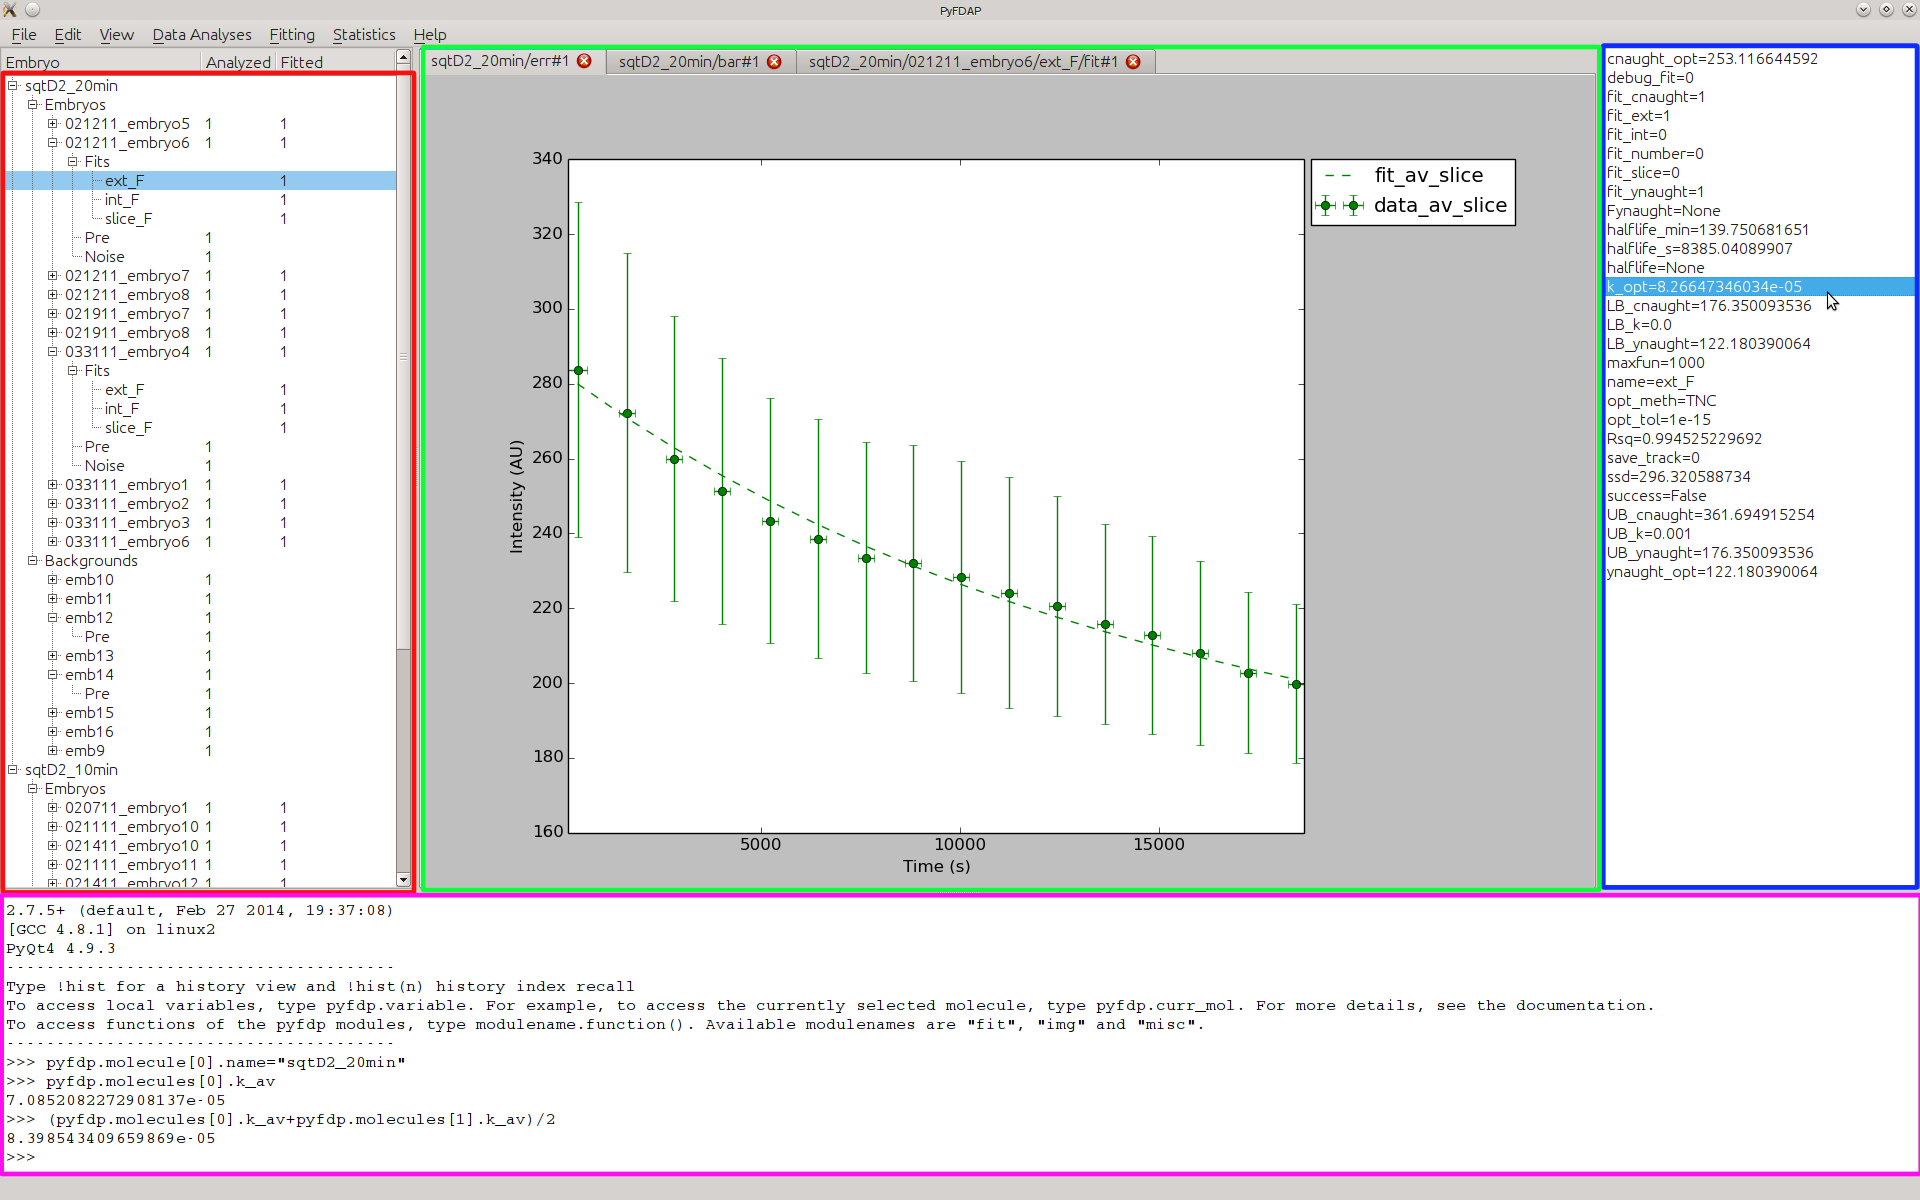
\includegraphics[scale=0.1925]{figs/pyfdp_mainframe_rect.png}
 \end{figure}

\noindent After creating a new molecule, FDAP, background dataset, or fit, the newly created object is shown in the object list according to its hierarchical structure (see Section~\ref{sec:structure}). To inspect the object properties, double-click on the object of choice. The object properties are then listed in the property list on the right-hand side. Many functions in PyFDAP will require you to select the right type of object and will return an error message if not done so.

PyFDAP provides the user with several plotting options. Each plot opens in a new tab with a name according to the currently selected object and the plot type. You can easily switch between plots by clicking on the open tabs. 

PyFDAP also comes with an internal Python console. NumPy and the three main PyFDAP modules \textit{img, fit, misc} are automatically imported. You can use the console to manipulate all PyFDAP objects such as molecules and embryos (FDAP datasets), call other Python functions or simply let PyFDAP return molecule or embryo properties such as longer vectors that are not shown in the property list. PyFDAP also uses the console for debugging outputs, so having a look at the console is often useful.

All major PyFDAP functions can be found in the menu bar at the top of the PyFDAP window. The menus are sorted according to the normal workflow of FDAP experiment analysis.  

\subsection{First steps with PyFDAP} 
We provide a fully analyzed FDAP dataset on our website. If you wish to try out PyFDAP using this test dataset, go to \url{http://people.tuebingen.mpg.de/mueller-lab}, download the test dataset \textit{TestDataset.zip}, and unzip it to your PyFDAP folder. If you wish to put it somewhere else, you need to adjust some paths in the molecule file in PyFDAP later. You can now analyze the raw images of the test dataset or your own data (see Section \ref{sec:raw}), or you can load a pre-analyzed dataset (see Section \ref{sec:pre}).

\subsubsection{Analyzing an FDAP dataset}
\label{sec:raw}
The following section guides you through the major steps of how to use PyFDAP to analyze and fit FDAP datasets if you wish to perform your own FDAP analysis.

\newcommand{\imgscale}{0.3}

\begin{enumerate}
 \item Create a new molecule project by clicking on \textit{File $\rightarrow$ New Molecule}.
 \begin{figure}[H]
  \centering
  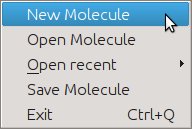
\includegraphics[scale=\imgscale]{figs/new_molecule.png}
 \end{figure}

 \item Change the name of the molecule project by clicking on \textit{Edit $\rightarrow$ Edit Molecule}.
 \item Add a new embryo object (FDAP measurement):
 \begin{enumerate}
 \item Go to \textit{Data Analyses $\rightarrow$ Embryo $\rightarrow$ New Embryo}
 \begin{figure}[H]
  \centering
  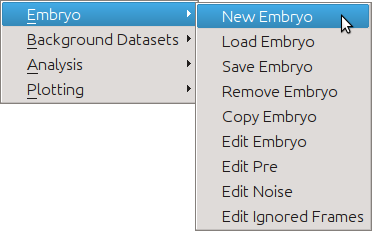
\includegraphics[scale=\imgscale]{figs/new_embryo.png}
 \end{figure}
 \item Choose the photoconverted folder (images of photoconverted proteins) and counter-labeled folder (images of cell-tracing molecules, e.g. Alexa488-Dextran). For the test dataset, these can be found in the folder \textit{TestDataset/squint-dendra2\_20min-interval/embryo6/post}; the photoconverted folder is called \textit{red}, and the counter-labeled folder is called \textit{green}.
 \item Enter the dataset-specific properties such as intervals between images (20 min = 1200~s for the test dataset), post-delay (delay between first and second post-conversion pictures resulting from re-adjustment), and center and radius for each image. You can easily select the center and the radius for each image by clicking on the picture. The first click will define the center, the second the radius, and the third click will delete both selections. If you wish to copy the selected radius and center for all following images, click on \textit{Copy geometry for following images}. When you are done defining the dataset, click on \textit{Done}.
  \begin{figure}[H]
  \centering
  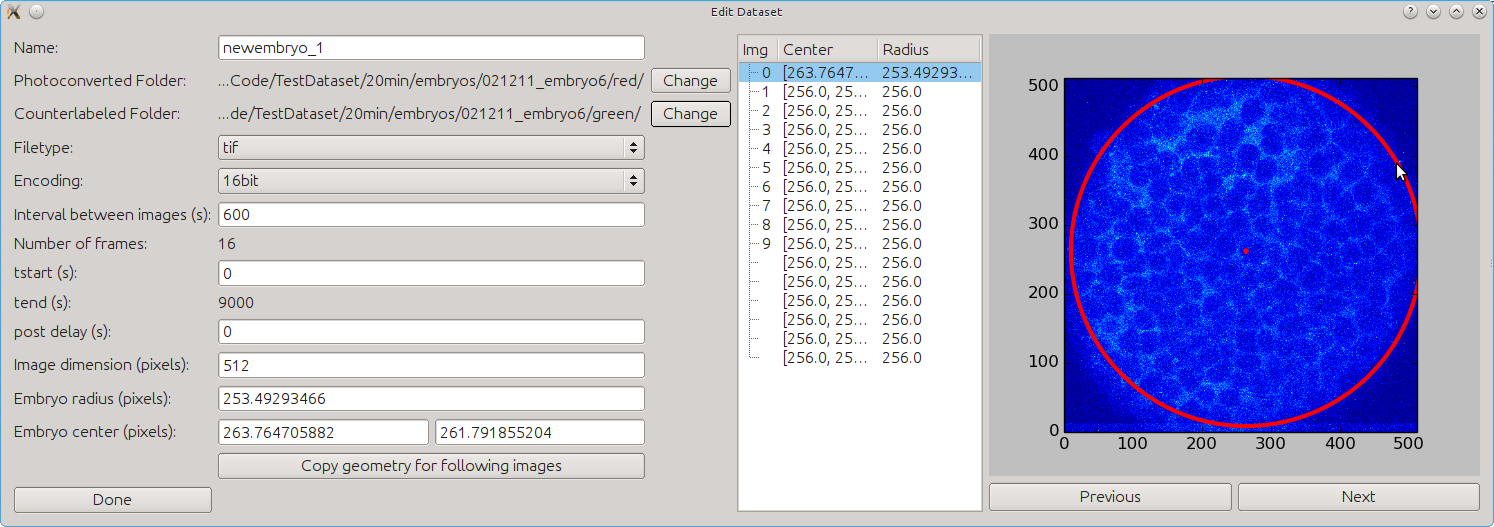
\includegraphics[scale=0.2]{figs/edit_embryo.png}
 \end{figure}
 \item The next pop-up window will allow you to set the ``photoconverted'' folder, counter-labeled folder, and specific properties of the pre-conversion images similar to the post-conversion dataset in steps (b) and (c). For the test dataset, these can be found in \textit{TestDataset/squint-dendra2\_20min-interval/embryo6/pre}; the ``photoconverted'' folder is called \textit{red}, and the counter-labeled folder is called \textit{green}.
 \item The third pop-up window will allow you to define the method of noise calculation. You can choose between three methods:
 \begin{itemize}
  \item \textit{Outside} will average intensities outside of the selected radius for each image defined in (c) and then average over all of the calculated averages.
  \item \textit{Predefined} gives you the possibility to enter a value for the noise level yourself.
  \item \textit{Separate Dataset} lets you analyze a separate dataset taken to calculate noise levels. These images are generally taken before or after the experiments without a sample. 
 \end{itemize}
 After clicking \textit{Done}, all important settings for the embryo object are entered.
\item You can add additional embryo objects (FDAP measurements) to the molecule by repeating steps (a) - (e). 
 \end{enumerate}
 \item Add a new background object:
 \begin{enumerate}
 \item Go to \textit{Data Analyses $\rightarrow$ Background Datasets $\rightarrow$ Add background dataset}.
  \begin{figure}[H]
  \centering
  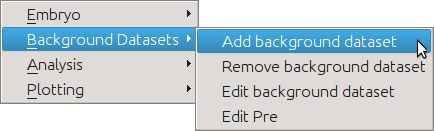
\includegraphics[scale=\imgscale]{figs/new_bkgd.png}
 \end{figure}
 \item Choose the ``photoconverted'' folder (images of ``photoconverted'' proteins) and counter-labeled folder (images of cell-tracing molecules). For the test dataset, these can be found in \textit{TestDataset/squint-background\_20min-interval/embryo10/post}; the ``photoconverted'' folder is called \textit{red}, and the counter-labeled folder is called \textit{green}.
 \item Similar to the embryo object, select parameters specific to the dataset by using the given text fields or by clicking on the image.
\item The next pop-up window will allow you to set the folders and properties of the pre-conversion images of the background dataset similar to the post-conversion dataset. For the test dataset, these can be found in \textit{TestDataset/squint-background\_20min-interval/embryo10/pre}; the ``photoconverted'' folder is called \textit{red}, and the counter-labeled folder is called \textit{green}.
\item  After clicking \textit{Done}, all important settings for the background object are entered. You can add additional background objects to the molecule by repeating steps (a) - (d). 
 \end{enumerate}
\item Analyze the molecule project by going to \textit{Data Analyses $\rightarrow$ Analysis $\rightarrow$ Analyze Molecule}. This can take several minutes depending on the amount of datasets added to the molecule project (see Section \ref{sec:performance}).
 \begin{figure}[H]
  \centering
  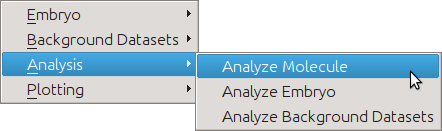
\includegraphics[scale=\imgscale]{figs/analyze_mol.png}
 \end{figure}
 The image analysis progress will be printed into the PyFDAP console.
\item Double-click on the embryo object you want to analyze and add a new fit object:
\begin{enumerate}
 \item Go to \textit{Fitting $\rightarrow$ Fits $\rightarrow$ New fit}.
 \item Enter the parameters of the fit. The most important are:
\begin{itemize}
 \item \textit{opt\_meth} is the optimization method (see Table \ref{tab:algorithms} for details) used for finding the minimum of the SSD (sum of squared differences).
 \item \textit{opt\_tol} is the level of tolerance (i.e how good the fit needs to be) given to the optimization algorithm.
 \item \textit{maxfun} is the maximum number of iterations used by the optimizer.
 \item \textit{Model} is the underlying decay model used for the fit. See Section \ref{sec:models} for more information.
 \item \textit{x0\_k, x0\_c0, x0\_y0} are the initial guesses for the three parameters $k$, $c_0$, and $y_0$.
 \item \textit{LB\_k, UB\_k, LB\_c0, UB\_c0, LB\_y0, UB\_y0} are the lower and upper bounds for the three parameters $k$, $c_0$, and $y_0$ given to the optimizer. You can use the checkboxes to set each variable bounded or unbounded from below and above. For the lower bound of $y_0$, PyFDAP offers several presets:
 \begin{itemize}
 \item \textit{Custom} allows you to enter a value yourself.
 \item \textit{Noise} takes the level of noise as the lower bound for $y_0$. 
 \item \textit{Bkgd\_pre} takes the level of the background pre-conversion images as the lower bound for $y_0$. 
 \item \textit{Bkgd} takes the average background level as the lower bound for $y_0$. 
 \item \textit{F} takes the weighting function given in \cite{Mueller2012} as the lower bound for $y_0$. 
\end{itemize}
More details on the estimation of initial guesses and variable bounds can be found in Section \ref{sec:bounds}. Note that not all optimization algorithms offer bounded optimization (see Section \ref{sec:algorithms} for more details). 
\item \textit{fit\_ext, fit\_int, fit\_slice} define which regions of the images need to be fitted. You can only select one of the three regions intracelluar, extracelluar, and slice (i.e. total imaged domain) to be fitted during one particular fit.
\item \textit{fit\_c0, fit\_y0} are flags on which parameters are kept fixed and which are free. If a parameter is unchecked, the optimization algorithm will keep this parameter at its initial guess value.
 \begin{figure}[H]
  \centering
  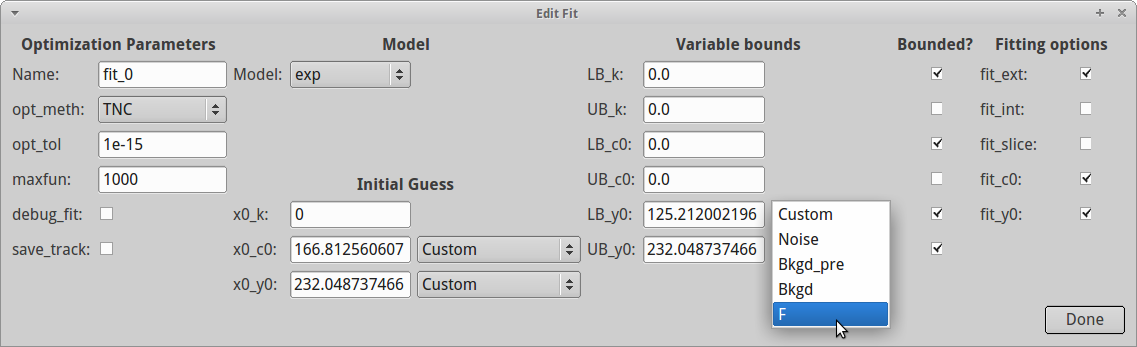
\includegraphics[scale=0.2]{figs/new_fit.png}
 \end{figure}
\item  After clicking \textit{Done}, all important settings for the fit object are entered. The fit is performed instantly, and you will see the fitted data. To inspect the optimal parameters resulting from the fit, double-click on the current fit and look in the property list on the right-hand side for \textit{k\_opt} (the decay rate constant) and \textit{halflife\_min} (the half-life in minutes). 
\begin{figure}[H]
  \centering
  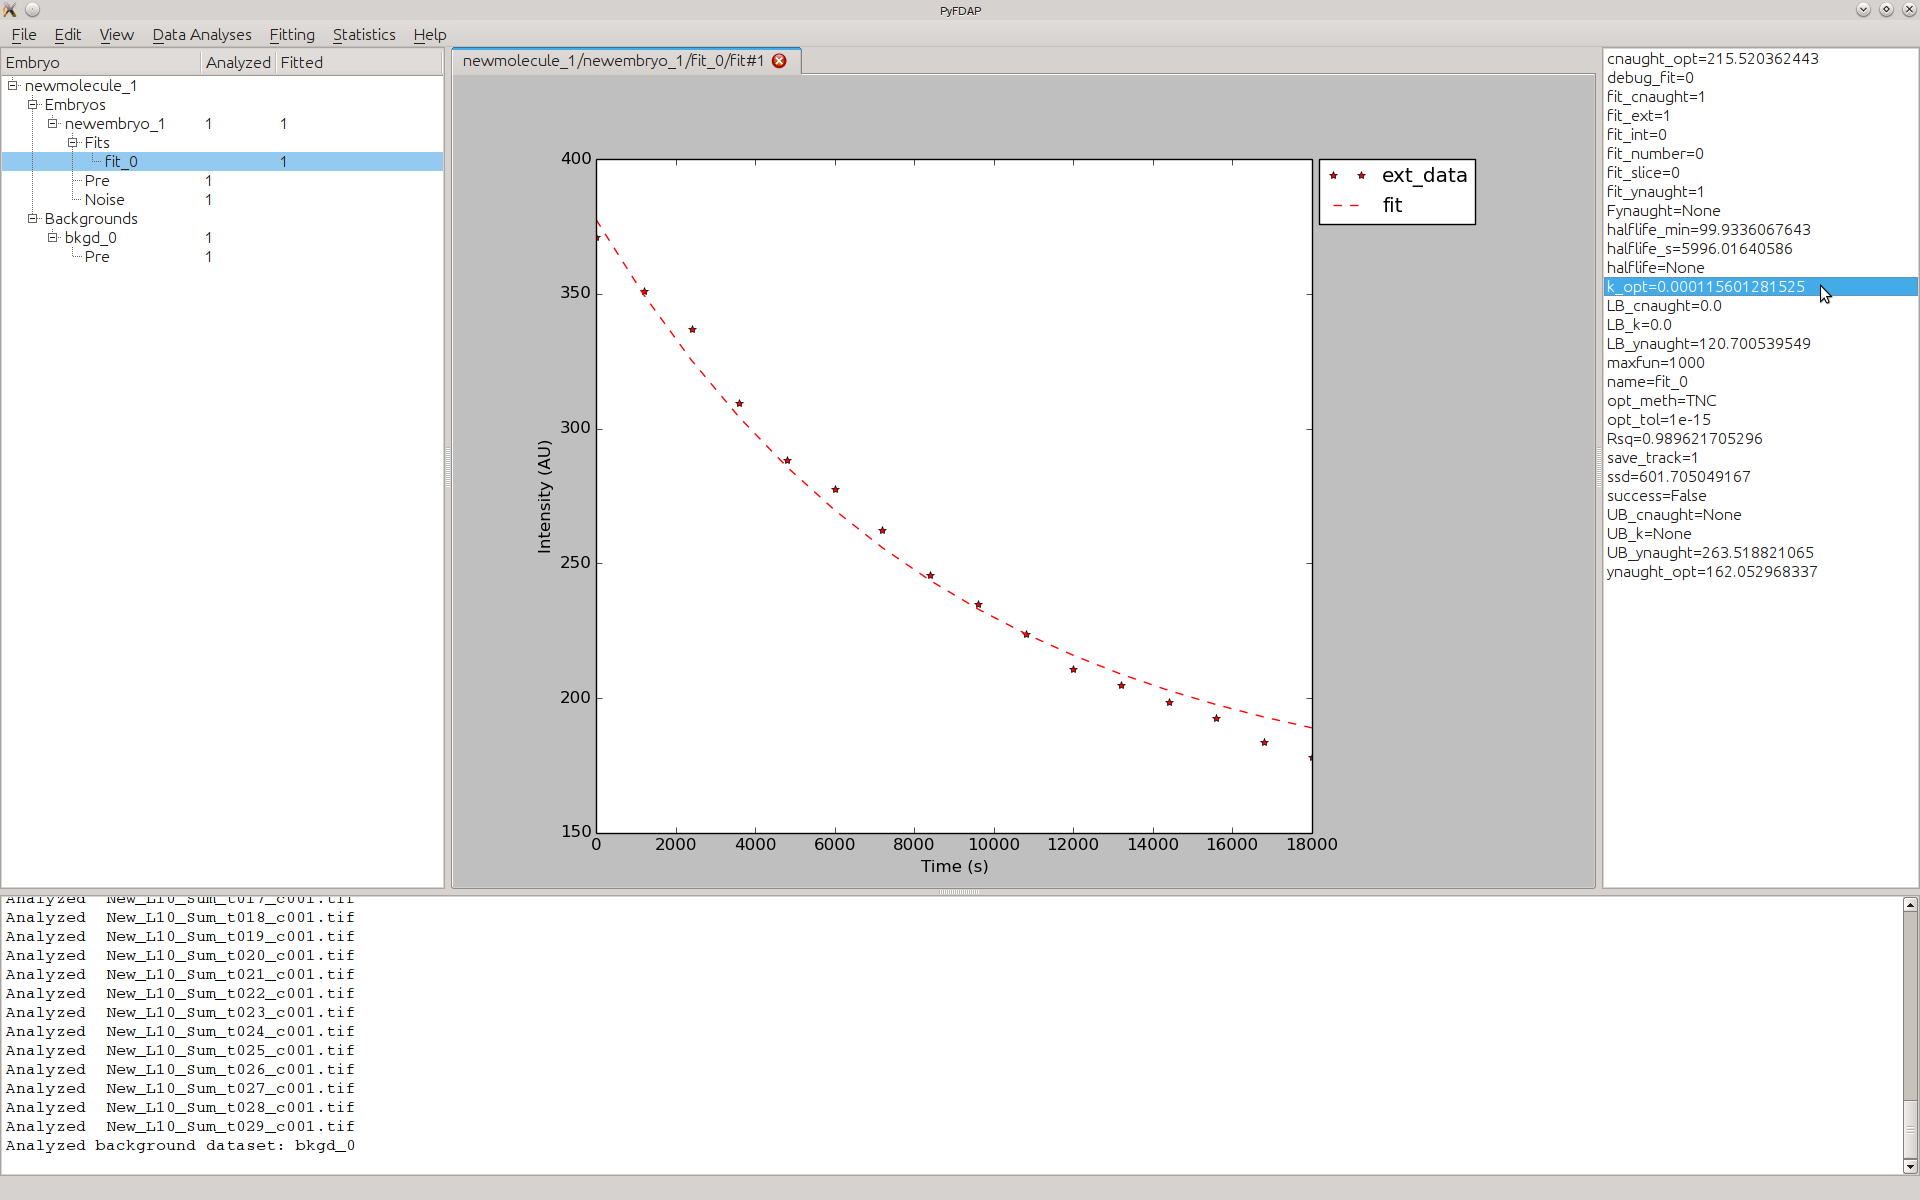
\includegraphics[scale=0.19]{figs/fit_done.png}
 \end{figure}
\end{itemize}
\item You can add additional fit objects to the molecule project by repeating steps (a) and (b) described above. 
 \end{enumerate}
 
\item If you changed any settings of a fit (by selecting \textit{Fitting $\rightarrow$ Fits $\rightarrow$ Edit fit}) and want it to be performed again, select the fit in the left column and go to \textit{Fitting $\rightarrow$ Perform Fits $\rightarrow$ Perform fit}.
\item If you have added and fitted multiple embryo objects (FDAP measurements) and wish to find the average fit over all embryo objects, go to \textit{Statistics $\rightarrow$ Plotting $\rightarrow$ Plot average fit} (see Section \ref{sec:average} for details).
\end{enumerate}

\subsubsection{Loading a pre-analyzed dataset}
\label{sec:pre}
Launch PyFDAP, go to \textit{File} $\rightarrow$ \textit{Open Molecule}, and select the file \textit{TestDataset/results/TestDataset\_20min.pk}. You have now successfully loaded a molecule project including one embryo object (FDAP dataset) and one background dataset. You can now try out all features of PyFDAP including all plotting functions. 

\subsection{Making use of statistical functions in PyFDAP}
\label{sec:average}

PyFDAP comes with a few statistical tools for data averaging and analysis. To average the fits from multiple embryo objects (FDAP measurements), go to \textit{Statistics $\rightarrow$ Average Molecule}. A pop-up window will ask you to select fits from different embryo objects: 
\begin{figure}[H]
  \centering
  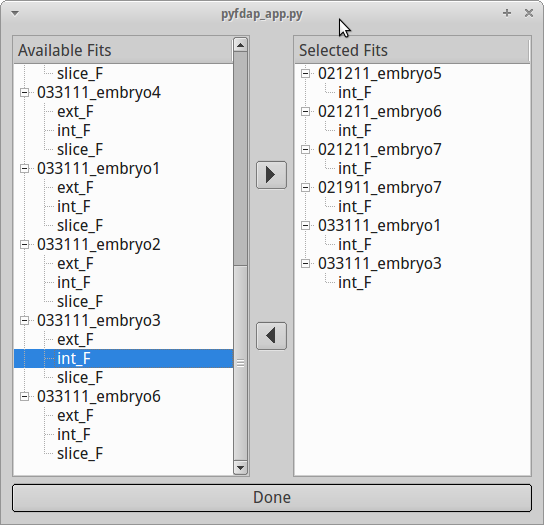
\includegraphics[scale=0.25]{figs/sel_fits.png}
 \end{figure}
\noindent You can add the fits that you want to be considered for averaging to the selection on the right-hand side by double-clicking on the particular fit or by using the arrow buttons on the screen. You can also remove fits from the selection by double-clicking or by using the arrow buttons. Note that for averaging to work, you can only select fits of the same region, e.g. you cannot average a fit for the extracellular region with one for the intracellular region. It is also not possible to let two fits of the same embryo object contribute to the averaged fit.

After selecting the fits that you want to include for averaging, press \textit{Done}. PyFDAP will automatically compute averages of all important fitting parameters and display them in the property list on the right-hand side. Details on how these averages are computed can be found in Section~\ref{sec:stats}. After averaging a selection of fits, you can use PyFDAP's bar plot functions to compare fitting results from different embryos. Go to \textit{Statistics $\rightarrow$ Plotting} and choose between \textit{Plot ks by fit}, \textit{Plot y0s by fit}, \textit{Plot c0s by fit} to plot each of the parameters by fit in a bar plot, or choose \textit{Plot all parameters by fit} to plot all three optimal parameters by fit. 
\begin{figure}[H]
  \centering
  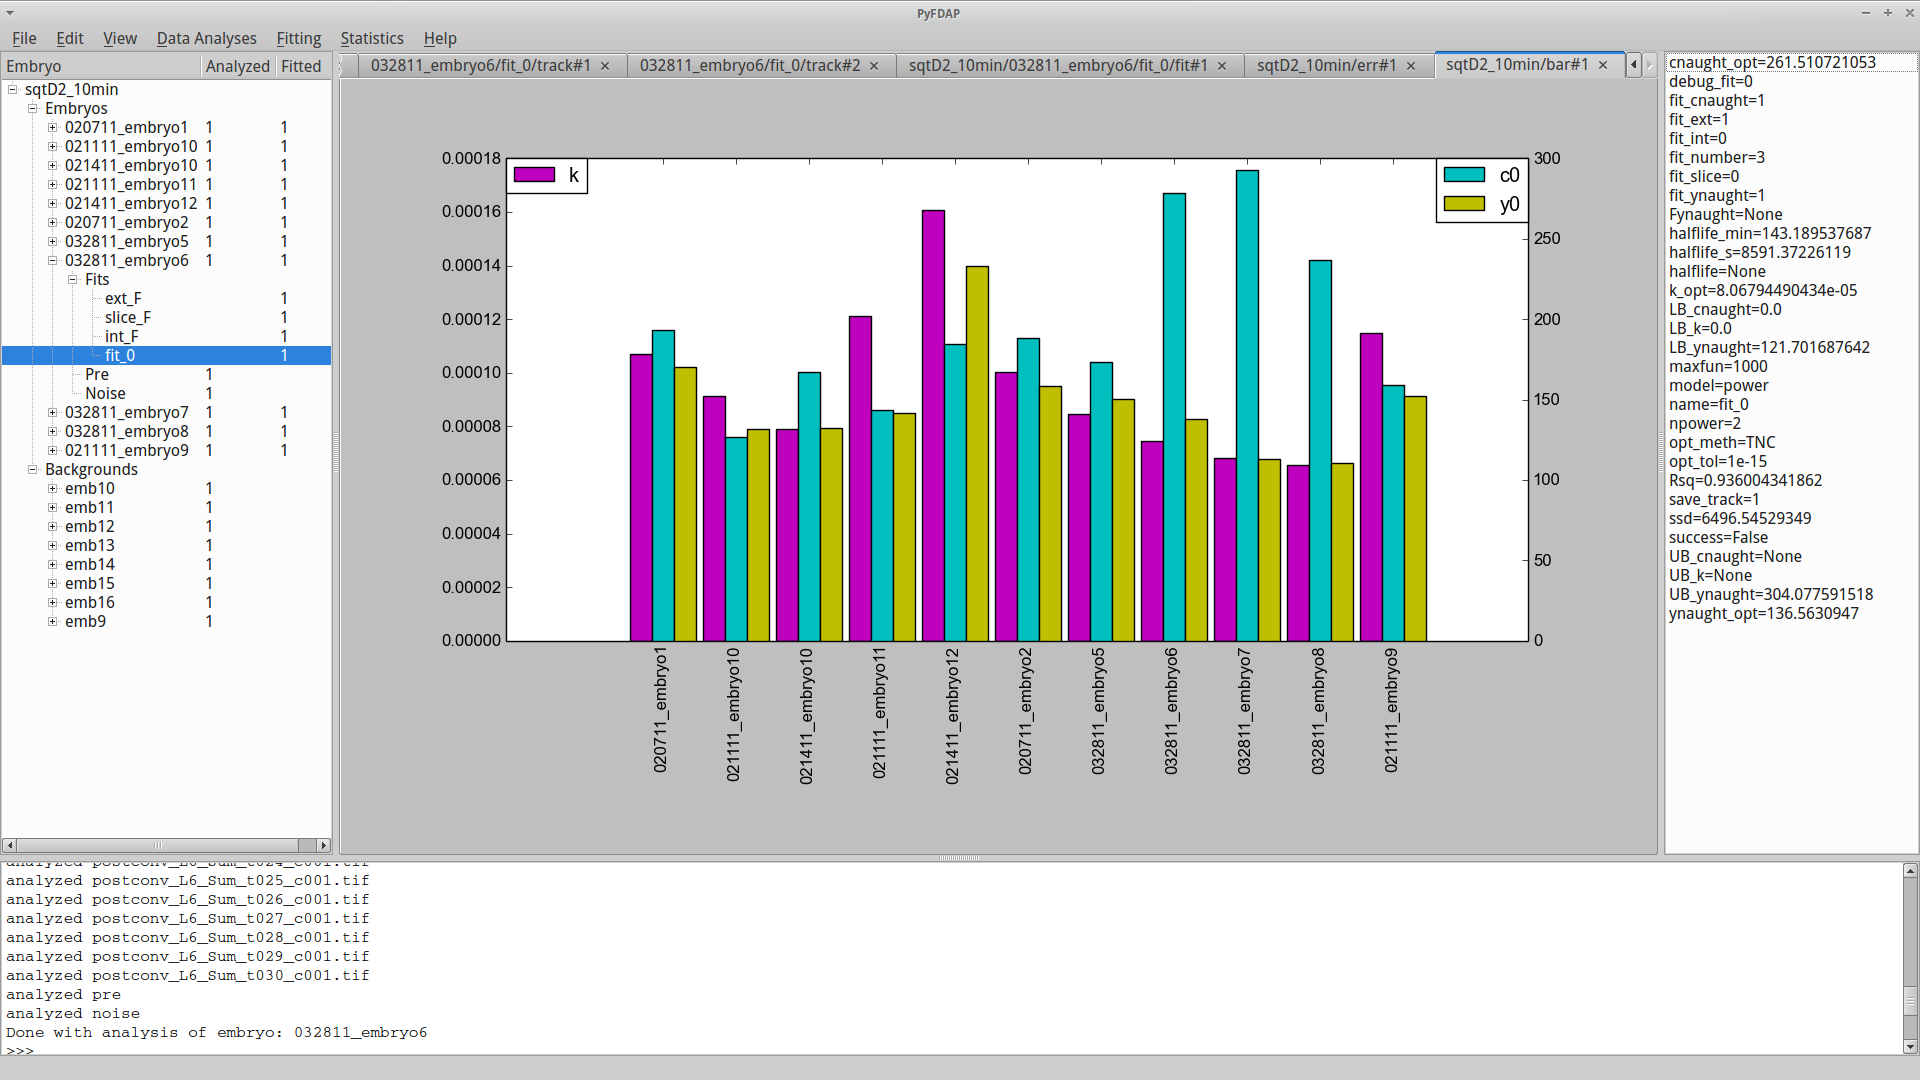
\includegraphics[scale=0.18]{figs/all_parameters.png}
 \end{figure}

\noindent This plot allows you to identify fits that produce parameters strongly deviating from the mean. You can then go  back to those fits and adjust the fitting parameters to optimize your final result.

You can also plot the averaged time-dependent fluorescence decay data as error bar plots for unnormalized data or for data normalized between values of $0$ and $1$. To generate these plots, go to \textit{Statistics $\rightarrow$ Plotting $\rightarrow$ Plot average fit} or \textit{Statistics $\rightarrow$ Plotting $\rightarrow$ Plot normed average fit}.  

\begin{figure}[H]
  \centering
  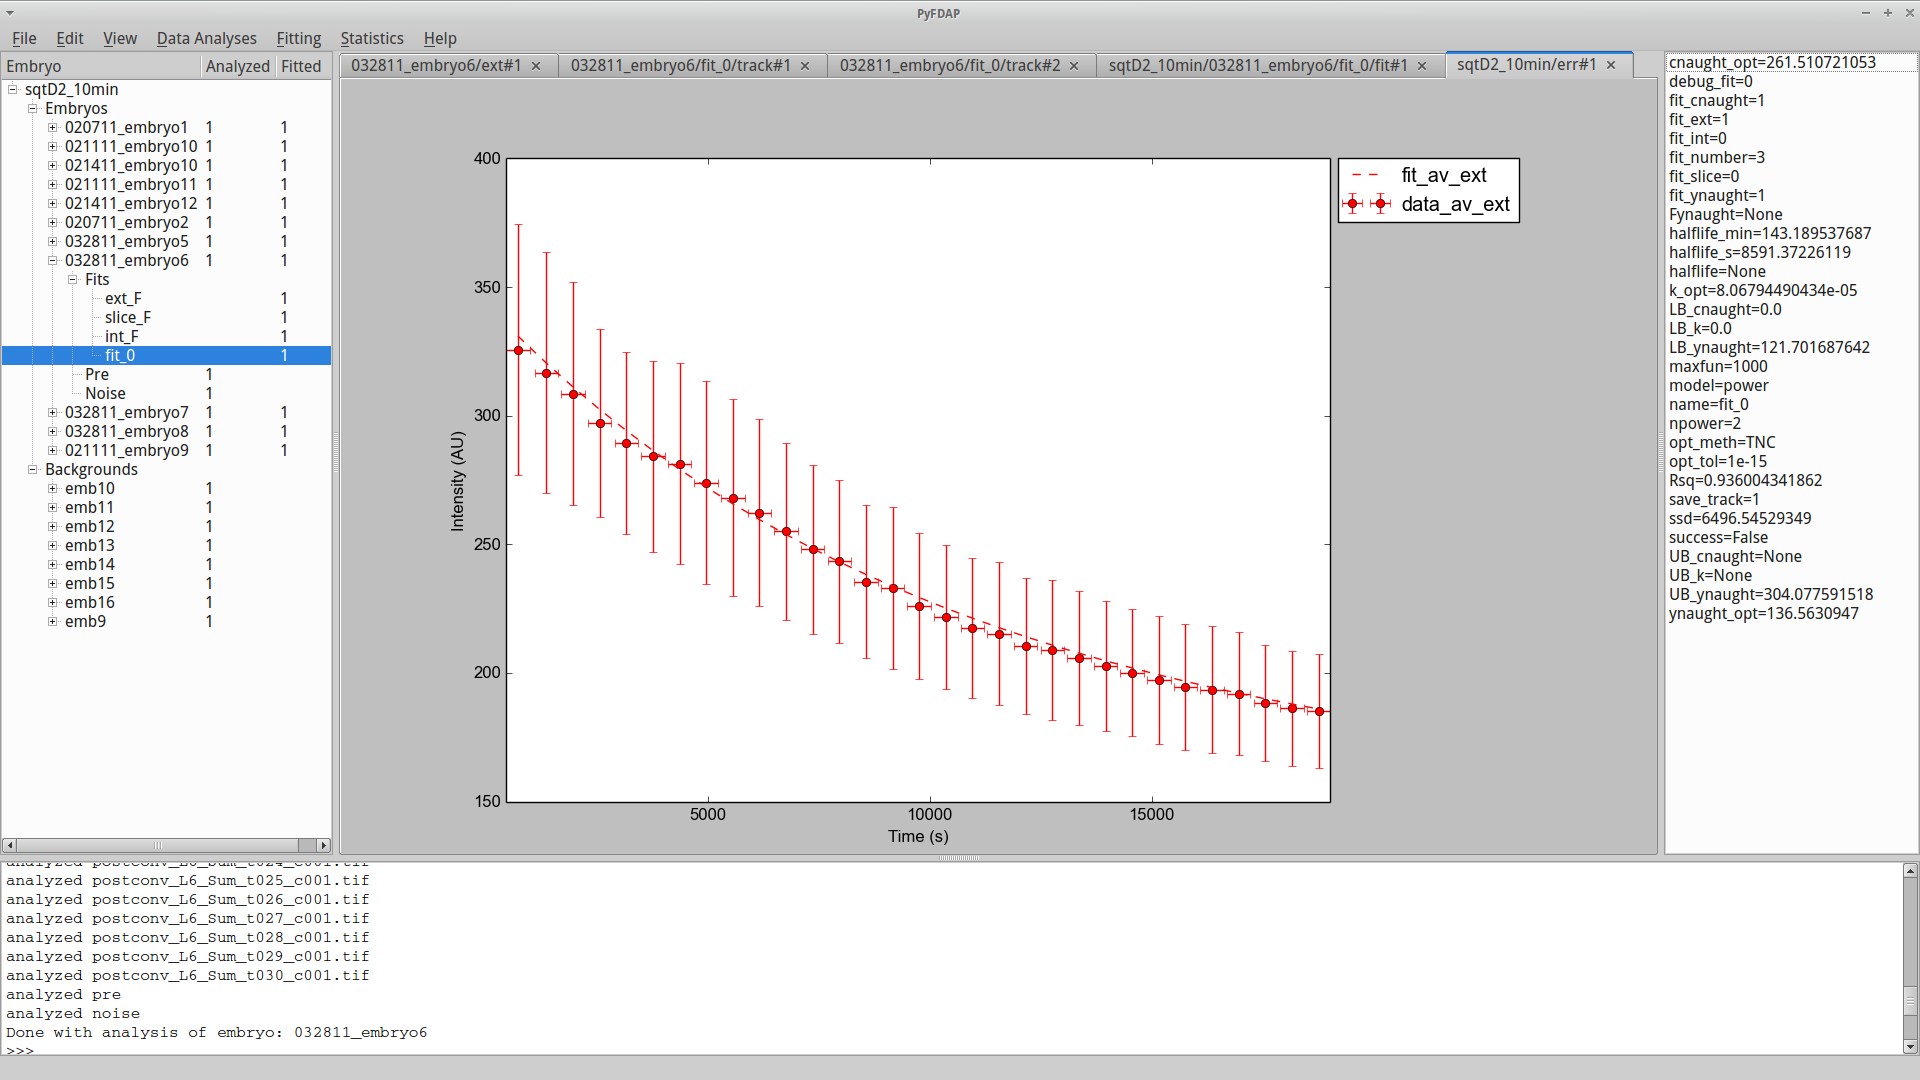
\includegraphics[scale=0.18]{figs/error_bar.png}
 \end{figure}

\noindent Mathematical details for error bar computation and data normalization can be found in Section \ref{sec:stats}.

\subsection{Saving results from PyFDAP}
\label{sec:output}
PyFDAP offers multiple ways to save and share FDAP project data and details such as plots, videos, analysis settings, and whole molecule projects. 

\subsubsection{Saving figures and movies}
\label{sec:movie}
In \textit{Data Analysis} $\rightarrow$ \textit{Plotting}, users can find plotting commands for
\begin{itemize}
 \item Data and background images for the whole region (slice) as well as for extra- and intracellular domains
 \item Masked images for the whole region (slice) as well as for extra- and intracellular domains
 \item Masks for the whole region (slice) as well as for extra- and intracellular domains
 \item Analysis results for all three regions including background values
\end{itemize}

\noindent Moreover, users can plot fitting results and the fitting progress under \textit{Fitting} $\rightarrow$ \textit{Plotting}. Single plot frames can be saved as *.png, *.pdf, *.eps, *.jpg, *.pgf, *.ps, *.rgba, *.svg, or *.tif. In order to edit the plots using a vector graphics software, we recommend saving images as *.pdf or *.eps files.

PyFDAP also allows users to export image series (such as the fitting progress) as *.mpg or *.avi movies for presentation purposes. Note that PyFDAP does not automatically provide the necessary package for the conversion of image files to movie files; more information about the installation process to enable video output can be found in Section~\ref{sec:video}.

\subsubsection{Saving molecule and embryo files}
Users can save their molecule sessions to JavaScript Object Notation (JSON) object files. These object files follow the logical hierarchical structure explained in Section~\ref{sec:structure} and contain all of the data used for the FDAP analysis as well as the fitting results. The molecule and embryo files can be re-loaded into PyFDAP to enable researchers to continue working on a session and to facilitate collaboration among researchers in different locations.

\subsubsection{Saving plots and results as .csv files}
Plots as well as molecule and embryo objects can also be saved as comma-separated value files that can then be read into other plotting or analysis software such as Excel or Matlab. The molecule and embryo *.csv files follow the hierarchical system of the JSON files (see above). Note that image data will not be exported to *.csv files.

\section{Data structure}
\label{sec:structure}
PyFDAP provides a hierarchical object structure to organize the datasets obtained from FDAP experiments and to facilitate data navigation (Figure~\ref{fig:structure}).

\begin{figure} [H]
 \centering
 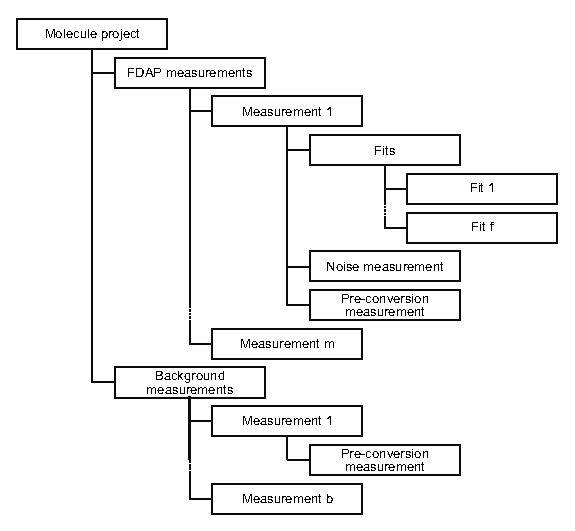
\includegraphics[scale=1.0]{figs/Blaessle_Figure1.eps}
\caption{Hierarchical PyFDAP data structure for FDAP experiments. Experiments are grouped into a main molecule project and divided into FDAP (1 to m) and background (1 to b) pre- and post-conversion measurements. Each FDAP measurement can have multiple fits (1 to f) with different fitting options.}
\label{fig:structure}
 \end{figure}

\noindent \textit{Molecule projects:} Replicate experiments with the same protein are grouped into a main molecule project. PyFDAP can handle multiple molecule projects in one session.  \\

\noindent \textit{FDAP measurements:} Replicate experiments are divided into FDAP and background pre- and post-conversion measurements. Intra- and extracellular protein stability can be different, and PyFDAP can import a second dataset that counter-labels intra- or extracellular space. The separation of fluorescence intensities into intra- or extracellular masks is performed using the Otsu binarization algorithm \citep{Otsu1979}. The masks and corresponding datasets can be investigated inside the PyFDAP GUI by clicking on \textit{Data Analysis} $\rightarrow$ \textit{Plotting} $\rightarrow$ \textit{Background Dataset}. The masks are applied to the images of the photoconverted signal, and the average intensities in the intra- and extracellular domains and in the entire image are calculated. Each PyFDAP embryo dataset (FDAP measurement) can have multiple fits for various regions, using different fitting parameters and different data points to allow maximum flexibility. The fits are automatically included in the PyFDAP data structure. \\

\noindent \textit{Noise measurements:} Noise measurements can be imported for each embryo dataset and can be used to calculate estimates for the baseline of the fit (see Section~\ref{sec:bounds}).\\

\noindent \textit{Pre-conversion measurements:} Pre-conversion intensity measurements provide information about the levels of autofluorescence and can be used to calculate estimates for the baseline of the fit (see Section~\ref{sec:bounds}).\\

\noindent \textit{Background measurements:} Background measurements provide information about the levels of autofluorescence after mock-photoconversion in the presence of unlabeled variants of the protein of interest and can be used to calculate estimates for the baseline of the fit (see Section~\ref{sec:bounds}).
 
\section{Performance}
\label{sec:performance}
We tested PyFDAP on various system configurations and ran a test script measuring the total operation time. The test script contained the following operations:

\begin{enumerate}
 \item Open a test molecule file
 \item Analyze a single FDAP dataset with all necessary additional data
 \item Analyze a background dataset with all necessary additional data
 \item Perform three fits for the intra- and extracellular and slice data
\end{enumerate}

\noindent The dataset used for this performance test is freely available from \url{http://people.tuebingen.mpg.de/mueller-lab/}, and the results of our performance tests are listed in Table~\ref{tab:time}.

\begin{table} [H]
  \small
  \centering
 \begin{tabular}{c|c|p{4cm}|c|c}
\textbf{System} & \textbf{OS} & \textbf{CPU} & \textbf{Memory} & \textbf{Operational Time} \\
 \hhline{=|=|=|=|=}
Thinkpad x230 & Xubuntu 14.04 & \centering Intel(R) Core(TM) i7-3520M, 2.90 GHz & 8 GB & 55 s \\
\hline
MacBookPro7.1 & Mac OS X 10.9.4 & \centering  Intel(R) Core(TM) 2 Duo-P8600, 2.40 GHz & 4 GB & 88 s \\
\hline
MacBookPro8.1 & Mac OS X 10.9.5 & \centering  Intel(R) Core(TM) i5-2410M , 2.30 GHz & 4 GB & 55 s \\
\end{tabular}
\caption{Performance test results of PyFDAP.}
\label{tab:time}
\end{table} 

\section{Mathematical background}

\subsection{Decay models}
\label{sec:models}
PyFDAP supports two different decay models: Linear- and non-linear decay. Linear decay is given by the ordinary differential equation (ODE)

\begin{equation*}
 \frac{\mathrm{d}c}{\mathrm{d}t} = -k c
\end{equation*}
\noindent where $c$ is the concentration of a molecule and $k$ is the rate constant of the decay. Since we assume that the level of fluorescence is proportional to the molecule concentration, we can substitute the concentration with fluorescence intensity. Solving this ODE results in 

\begin{equation*}
 c(t)=c_0 e^{-k t} + y_0
\end{equation*}
\noindent where $c(t)$ is the concentration of a molecule at time $t$, $c(0)=c_0$ is the concentration at time $t=0$, and $y_0$ is the baseline fluorescence intensity to which the population of decaying molecules converges. In terms of fluorescence intensity, $y_0$ resembles the baseline level of noise and autofluorescence. From $k$ we can then compute the molecule's half-life $\tau$ by
\begin{equation*}
 \tau= \frac{\ln(2)}{k}.
\end{equation*}

\noindent Some molecules are proposed to decay non-linearly \citep{Eldar2003}, and we have

\begin{equation*}
 \frac{\mathrm{d}c}{\mathrm{d}t} = -k c^n
\end{equation*}

\noindent where $n>1$ is the degree of non-linearity and $k$ is the decay rate constant of the molecule. We can solve this ODE and obtain the power-law solution

\begin{equation*}
 c(t)=\left(c_0^{1-n}  - kt(1-n)  \right)^{\frac{1}{1-n}}+ y_0.
\end{equation*}

\noindent For the case of a non-linear decay model, we compute the molecule's half-life by

\begin{equation*}
\tau=\frac{(2^{n-1}-1) c_0^{1-n}}{k(n-1)}.
\end{equation*}

\subsection{Estimation of initial guesses and bounds for variables}
\label{sec:bounds}
PyFDAP offers multiple options to calculate initial guesses and bounds for variables that are used by the fitting algorithms to obtain biologically reasonable estimates based on noise, pre-conversion, and background measurements (see Section \ref{sec:structure}).\\ 

\noindent \textit{Initial guess for the estimation of $c_0$:} A good estimate for $c_0$ is the difference between the pre-conversion and the first post-conversion image, i.e.

\begin{equation*}
 I_{\mathrm{post}}(t_{\mathrm{start}})-I_{\mathrm{pre}},
\end{equation*}

\noindent where $I_{\mathrm{post}}$ and $I_{\mathrm{pre}}$ are the fluorescence intensities after and before photoconversion, respectively, and $t_{\mathrm{start}}$ is the time at which the first image was taken. \\

\noindent \textit{Initial guess for the estimation of the baseline $y_0$:} PyFDAP offers the two presets $I_{\mathrm{post}}(t_{\mathrm{start}})$ and $I_{\mathrm{post}}(t_{\mathrm{end}})$, where $t_{\mathrm{end}}$ is the time at which the last image was taken and where protein decay should be almost complete. Our tests showed that the optimization algorithms worked well if $y_{0,\mathrm{opt}}$ is approached from above using $I_{\mathrm{post}}(t_{\mathrm{start}})$ as the initial guess for $y_0$.\\

\noindent \textit{Estimation of the lower bound for the baseline $y_0$:} This estimate is a crucial part of the fitting process. PyFDAP offers several algorithms to perform this estimation based on the amount and quality of the data available. 

\begin{itemize}

\item The simplest estimate of the lower bound of $y_0$ is the average background noise of the measurements $\bar{N}$. Due to autofluorescence of the samples, this estimate is generally too low, but it serves as the lower bound of the lower bounds of $y_0$.

\item Alternatively, the lower bound of the baseline $y_0$ can be estimated from the average level of autofluorescence represented by 

\begin{equation*}
 \bar{B}_{\mathrm{pre}_{r}} = \frac{\sum\limits_{j=1}^{b} B_{\mathrm{pre}_{j,r}}}{b},
\end{equation*}

\noindent where  $r\in \{\mathrm{intracellular,}$ $\mathrm{extracellular,}$ $\mathrm{entire \; domain}\}$ is the investigated region,  and $j \in \{ 1,...,b\}$ are the indices of background pre-conversion datasets with intensities $B_{\mathrm{pre}_{j,r}}$. 

\item PyFDAP also offers the possibility to use the average background intensity as the lower bound of the baseline $y_0$:

\begin{equation*}
 \bar{B}_{r} = \frac{\sum\limits_{j=1}^{b} \bar{B}_{j,r}}{b},
\end{equation*}

\noindent where $\bar{B}_{j,r}$ is the mean intensity in region $r$ of a background dataset over all data points given by 

\begin{equation*}
 \bar{B}_{j,r} = \frac{\sum\limits_{l=1}^{T} B(t_l)_{j,r}+ B_{\mathrm{pre}_{j,r}}}{T+1}.
\end{equation*}

Here, $t_l$ with $l\in \{1,...,T\}$ is the time when the $l$-th image was taken and $T$ is the number of post-conversion images.

\item PyFDAP includes a special weighting function $F$ \citep{Mueller2012} given by
\begin{equation*}
 F_{i,r} = \frac{1}{b}\sum\limits_{j=1}^{b} \min\limits_{t}\left(\frac{B_{j,r}(t)-N_i}{B_{\mathrm{pre}_{j,r}} - N_i} \right),
\end{equation*}
\noindent where $i$ is the current FDAP measurement, $r$ is the investigated region, and $j$ is the index of background datasets with intensities $B(t)$
at time $t$. Here, the noise measurement of measurement $i$ is given by $N_i$. Using the function $F$, users can compute the lower bound of the baseline $y_{{0}_{i,r}}$ for measurement $i$ and region $r$ by
\begin{equation*}
y_{{0}_{i,r}}\geq F_{i,r} \cdot (I_{\mathrm{pre}_{i,r}}-N_i)+N_i,
 \end{equation*}
\noindent where $I_{\mathrm{pre}_{i,r}}$ denotes the pre-conversion intensity of the FDAP measurement $i$ in region $r$.

\end{itemize}

\subsection{Optimization algorithms}
\label{sec:algorithms}
PyFDAP comes with a wide selection of optimization algorithms taken from the SciPy optimize package (\href{http://docs.scipy.org/doc/scipy/reference/optimize.html}{http://docs.scipy.org/doc/scipy/reference/optimize.html}) (\cite{Nelder1965,Polak1969,Broyden1970,Goldfarb1970,Fletcher1970,Shanno1970,Nash1984,Kraft1988,Byrd1995,Nocedal2006}). A list of all optimization algorithms available in PyFDAP can be found in Table \ref{tab:algorithms}.

\begin{table}
 \small
  \centering
 \begin{tabular}{p{4cm}|c|c|p{4cm}}

\textbf{Method} & \textbf{Name in PyFDAP} & \textbf{Type} & \textbf{Reference} \\
\hhline{=|=|=|=}
 \multicolumn{4}{c}{\textbf{Bounded methods}}\\
 \hline
\raggedright Limited-memory BFGS & L-BFGS-B &\centering quasi-Newton & \cite{Byrd1995} \\
 \hline
\raggedright Truncated Newton Conjugate & TNC &\centering Newton conjugate & \cite{Nash1984} \\
  \hline
\raggedright Sequential Least Squares Programming & SLSQP &\centering  sequential quadratic & \cite{Kraft1988} \\
 \hline
\raggedright Brute force & brute &\centering brute force & SciPy Reference Guide\\
 \hline
 \multicolumn{4}{c}{\textbf{Unbounded methods}}\\
  \hline
\raggedright Nelder-Mead & Nelder-Mead &\centering simplex & \cite{Nelder1965} \\
 \hline
\raggedright Broyden-\-Fletcher-\-Goldfarb-\-Shanno & BFGS &\centering quasi-Newton & \cite{Broyden1970,Goldfarb1970,Fletcher1970,Shanno1970}\\
 \hline
\raggedright Nonlinear Conjugate Gradient & CG &\centering Newton conjugate & \cite{Polak1969} \\
 \end{tabular}
\caption{List of optimization algorithms in PyFDAP.}
\label{tab:algorithms}
\end{table}

\subsection{Statistics}
\label{sec:stats}

PyFDAP can average over multiple fits from different embryo objects (FDAP measurements). Details of how to select fits for averaging are described in Section~\ref{sec:average}.

PyFDAP averages the optimal parameters for $k$, $y_0$, $c_0$, and protein half-lives $\tau$ through an arithmetic mean. For example, the average decay rate constant $\bar{k}$ is obtained by

\begin{equation*}
 \bar{k}=\frac{\sum\limits_{i=1}^{\tilde{m}} k_i} {\tilde{m}},
\end{equation*}

\noindent where $\tilde{m}$ is the number of fits to be averaged. The average half-life $\bar{\tau}$ can be computed in two ways resulting in different average
half-lives. PyFDAP computes the average half-life $\bar{\tau}$ through the arithmetic mean given by

\begin{equation*}
 \bar{\tau}=\frac{\sum\limits_{i=1}^{\tilde{m}} \tau_i} {\tilde{m}}.
\end{equation*}

\noindent For the linear decay model, this yields

\begin{equation}
\label{equ:lin_1}
 \bar{\tau}=\frac{1}{\tilde{m}}\sum\limits_{i=1}^{\tilde{m}} \frac{\ln(2)}{k_i},
\end{equation}

\noindent and in the case of the non-linear decay model we obtain

\begin{equation}
\label{equ:nonlin_1}
 \bar{\tau}=\frac{1}{\tilde{m}}\sum\limits_{i=1}^{\tilde{m}} \frac{(2^{n-1}-1) c_{0,i}^{1-n}}{k_{i}(n-1)}.
\end{equation}

\noindent However, computing the average half-life $\bar{\tau}$ directly from the average decay rate $\bar{k}$ yields 

\begin{equation}
\label{equ:lin_2}
 \bar{\tau}=\frac{\ln(2)}{\frac{1}{\tilde{m}}\sum\limits_{i=1}^{\tilde{m}} k_i},
\end{equation}

\noindent for the linear decay model and

\begin{equation}
\label{equ:nonlin_2}
 \bar{\tau}= \frac{(2^{n-1}-1) \frac{1}{\tilde{m}}\sum\limits_{i=1}^{\tilde{m}} c_{0,i}^{1-n}}{\frac{1}{\tilde{m}}\sum\limits_{i=1}^{\tilde{m}}k_{i}(n-1)}.
\end{equation}

\noindent in case of the non-linear decay model. It is obvious that equations \ref{equ:lin_1} and \ref{equ:lin_2} as well as equations \ref{equ:nonlin_1} and \ref{equ:nonlin_2} do not produce the same half-lives, and the user needs to decide which way of half-life computation is appropriate for the application.

PyFDAP can produce different error bar plots for each averaged region. Clicking on \textit{Statistics} $\rightarrow$ \textit{Plotting} $\rightarrow$ \textit{Plot average fit} will result in a plot in which each average data point $\bar{c}(t_j)$ is computed as the arithmetic mean

\begin{equation*}
\bar{c}(t_j)=\frac{1}{\tilde{m}}\sum\limits_{i=1}^{\tilde{m}} c_i (t_j).
\end{equation*}

\noindent Error bars are computed as the standard deviation for each time $t_j$. Clicking on \textit{Statistics} $\rightarrow$ \textit{Plotting} $\rightarrow$ \textit{Plot normed average fit} returns a plot in which all data points are normalized between values of $0$ and $1$. The normalization is performed by subtracting the baseline value $y_{0,i}$ from each data point and dividing the result by $c_{0,i}$, i.e.

\begin{equation*}
\tilde{c_i}(t_j)= \frac{c_i (t_j)-y_{0,i}}{c_{0,i}},
\end{equation*}

\noindent where $\tilde{c_i}(t_j)$ is the normalized data point at time $t_j$. This normalization facilitates the comparison of decay curve shapes, but it substantially changes the meaning of the error bars. Since all data series are pinned to a value of $1$ at their first time point, the standard deviation vanishes for this data point. The following data points will generally produce increasing error bars since the decay curves generally diverge. The length of the normalized error bars can be interpreted as the extent to which the decay curves diverge throughout the experiments.

\section{Acknowledgments}
We thank Katherine Rogers and Gary Soh for useful suggestions and for testing PyFDAP. We thank Katherine Rogers and Alex Schier for providing the test dataset.

\pagebreak

\section{List of frequently used abbreviations and variables}
\begin{tabular}{lll} 
\\
\toprule
\textbf{Name} & \textbf{Description}\\
\midrule
\\
\textbf{Abbreviations}\\
LB & Lower bound\\
UB & Upper bound\\
ODE & Ordinary differential equation\\
SSD & Sum of squared differences\\
\\
\textbf{Variables}\\
$b$ & Number of background measurements \\
$B$ & Background intensity \\
$c$ & Molecule concentration\\
$c_0$ & Initial molecule concentration \\
$\tilde{c}$ & Normalized molecule concentration \\
$f$ & Number of fits \\
$F$ & Weighting function for the estimation of the lower bound of $y_0$ \\
$i$ & Control variable \\
$I$ & Fluorescence intensity \\
$j$ & Control variable \\
$k$ & Molecule decay rate constant \\
$l$ & Control variable \\
$m$ & Number of measurements \\
$\tilde{m}$ & Number of selected fits for averaging \\
$n$ & Degree of non-linearity of molecule decay \\
$N$ & Noise intensity \\
$r$ & Region of measurement \\
$t$ & Time \\
$T$ & Number of post-conversion frames \\
$\tau$ & Molecule half-life \\
$x_0$ & Initial parameter guess\\
$y_0$ & Molecule decay baseline \\
\\
\textbf{Variable subscripts}\\
$ext$ & Extracellular\\
$int$ & Intracellular\\
$post$ & After photoconversion\\
$pre$ & Before photoconversion\\
$slice$ & Entire optical slice\\
\bottomrule
\end{tabular}

\pagebreak

\bibliographystyle{natbib}
\bibliography{Blaessle_PyFDAP}

\end{document}